%% APPENDIX B -- the spatial rank as a diagnostic: what it can and cannot
%% support, and the reserved hold-out that calibrates it.
%% Owner: r11-chain.  Carries \label{app:radius} (cited by 04_method.tex)
%% and \label{sec:heldout} (cited from the other appendices).
\section{The spatial rank, and what it can support}
\label{app:radius}

The spatial rank asks whether an excess sits at the star or anywhere else in
the field. It is a diagnostic, no disposition rests on it, and this appendix
is the measurement that settles why: \rankstatus{}

The star lies at the phase centre, inside the control annulus, and the
asymmetry is real. \emph{It is not a primary-beam effect.} Spectra are
extracted from phase-rotated visibilities in apparent flux and are never
corrected for the primary-beam response (Appendix~\ref{app:conventions}), so
the familiar rise of image noise with distance from the pointing centre
cannot operate here; and were it operating, it would make the control probes
noisier than the star and place the stellar rank \emph{above} one half, the
opposite of what is measured. No mechanism for the displacement is
established. What the control ensemble does show is
a weak rise of its own level with radius, and the obvious repair is to remove
it: each probe is standardised within its own radius bin, the radii being
known from the fixed draw, with no free parameter.

\emph{Applied out of sample, the correction does not repair the statistic.}
Frozen --- probe radii, bin edges and standardisation alike --- and applied
unmodified to \RadValStarN{} windows that played no part in its construction,
it moves the median stellar rank from \RadValStarRawMed{} to
\RadValStarCorMed{} against the exchangeable one half, \RadValStarToward{}
it, in both out-of-sample partitions separately. Rescoring the whole survey
with the gradient removed moves the list of crossings outranking all their
controls from \LocStageGlobal{} windows to \LocStageLocal, losing
\LocStageLost{} and gaining \LocStageGained, and leaves the survey median
rank slightly further from one half than before.

The radial gradient is real, but removing it leaves the median no closer to
one half, so the residual is not radial and neither normalisation yields a
calibrated tail probability. We therefore keep the frozen rank, read
it only as an indication of which crossing to examine first, and rest every
disposition on physical evidence or on recurrence. The radial correction, the
region-maximum audit and the pseudo-star tests each leave every disposition
unchanged, and because the rank gates nothing, none of this enters a
sensitivity limit.

\emph{One mechanism can be excluded by measurement, and it is the one that
would matter most.} Equation~\ref{eq:tstar} divides every position by a
single noise scale shared by the star and all its probes. A star bright
enough to carry multiplicative calibration residuals of its own would then
have a noise the shared scale does not describe, and its statistic would be
inflated with nothing in the search to reveal it. The ratio of the two noises
is measurable from the released control vectors alone: because the star and
each probe are divided by the same scale and maximised over the same
channel$\times$drift grid, the stellar statistic divided by the median of
the \NCtrl{} control statistics \emph{is} that ratio, and it is one when the
two noises agree. Over the \NsrNWin{} windows carrying no threshold crossing
its median is \NsrMed{} (star-clustered 95 per cent \NsrLo--\NsrHi), and it
does not climb with the brightness of the field, which is what a
multiplicative error would scale with: \NsrFifthLo{} in the faintest fifth of
control rings against \NsrFifthHi{} in the brightest, and \NsrBrightMed{}
over the \NsrBrightN{} windows whose ring exceeds \NsrBrightSig$\sigma$ and
is therefore set by resolved emission rather than noise. That the ratio
\emph{can} rise is shown by the \NsrCrossN{} windows that do carry a
crossing, where it is \NsrCrossMed. Part of the reason it does not rise
otherwise is structural: a gain error multiplying a continuum raises every
channel of an integration by the same factor, and the per-integration median
along frequency removes exactly that. \textbf{A stellar-position noise
denominator would therefore move no statistic in this survey.}

\subsection{The reserved hold-out, and what it calibrates}
\label{sec:heldout}

The statistic and the mask were settled on the searched sample and cannot also
calibrate themselves, so a hold-out was reserved by a rule fixed and recorded
before any reserved block was searched: a block is held out if and only if
$\mathrm{sha256}(\textsc{uid})_{[:8]} \bmod 5 = 0$, subject to two guards that
use identifiers alone --- a block on the pre-registered list deposited with
this paper stays in the survey, and no system loses every block --- so that
the assignment can be recomputed from the UIDs and that list alone. The
statistic, the trigger and the recurrence criterion were all fixed before the
rule itself, and the first reserved block was searched \HoLeadBlockDays{} days
later, so every diagnostic built afterwards is incapable of promoting a
window. Of \NEbProcessedAll{} blocks processed, \NEbHeldOut{} are reserved
(\HoPctHeld{} per cent), giving \HoWin{} windows toward \HoStars{} stars with
no star and no system lost from the headline sample. Three quantities are
calibrated on those blocks and on nothing else.

First, the rank displacement. Out of sample the stellar rank has median
\HoRankMed{} where one half is expected, with a block-clustered 95 per cent
interval of \HoRankMedLo--\HoRankMedHi{} over \HoWin{} windows, and
\HOFracLoPct{} per cent of ranks below 0.1 against \HOFracHiPct{} per cent
above 0.9, so the distribution is displaced rather than growing a tail. The
displacement runs the way that matters: a rank below one half places the star
high, and the star in fact outranks all \NCtrl{} probes in \NsrFirstObs{} of
the survey's windows against \NsrFirstExp{} if the positions were
interchangeable. The direction therefore inflates star-first outcomes rather
than suppressing them, which is why the chance expectations of
Appendix~\ref{app:falsealarm} are calibrated on the measured rate.
Clustering removes neither the shift nor its size: \HOBlockBelow{} of
\HOBlockN{} blocks have a mean rank below 0.5, and a star-clustered bootstrap
places the median at \HOBootMed{} (95 per cent \HOBootLo--\HOBootHi). The
searched sample leans the same way but by less (median \SurvMedP,
star-clustered 95 per cent \SurvBootLo--\SurvBootHi), and the two
intervals do not overlap, so the displacement is a property of these
reserved blocks and is not reproduced in sample. Either way it runs in the
direction that inflates star-first outcomes, which is the quantitative
reason the rank is read as a diagnostic and never as a significance.

Second, the false-alarm tail factor --- the measured rate at which a
no-signal position ranks first, divided by the rate exchangeability would
give. It is \HoTailFactor{} on \HoPseudoTrials{} trials, with a bootstrap
clustered over the \HoTailBlocks{} reserved blocks giving
\HoTailLo--\HoTailHi. It is a statement about the rank and not about the
trigger, so it is reported as a diagnostic; the quantity the chance
expectations need is the exceedance rate at the stellar position, measured
on the same blocks in Appendix~\ref{app:falsealarm}.

Third, the radial behaviour of the control ensemble: the standardised level
runs \HoRadBins{} across the annulus, a mean per-window slope of
$\HoRadSlope\pm\HoRadSlopeSe$, small and of the wrong sign to account for the
displacement.

The \emph{external calibration sample} must not be confused with the
hold-out, and it is not an out-of-sample set. Its \CampBlocks{} execution
blocks were reserved to calibrate the rank and to supply repeats the hold-out
does not have, and \CalNCensus{} of them are primary-census blocks and
\CalNHoldout{} hold-out blocks, with \CalNOutside{} outside both: it enters no
count of the science sample because its blocks are already counted there, not
because it is external. Over its \CampWindows{} windows the frozen pipeline
returns \CampStageOne{} crossings outranking all their controls ---
\CampStageOneCO{} of them $\beta$~Pictoris CO --- and \CampUnattrib{}
unattributed against \CampExpUn{} expected at the measured tail rate.

\subsection{One crossing through the whole chain}
%% (subsection label retired: nothing cites it)

CP$-$72~2713 is the clearest worked example, because every step returns a
verdict rather than a shrug. In Band~7 the crossing reaches
$T_\star=\VnCpT$ in channel \VnCpChan{} of its window; it is unattributed,
with the one nearby transition and its provenance discussed in
Appendix~\ref{app:linemask}; both diagnostics favour it, in that it outranks
every one of the \NCtrl{} control positions and the drift-following
visibility fit puts the emission at the stellar position, ${\rm
Re}/\sigma=\VnCpReAdopted$ against a control-position maximum of
\VnCpCtrlAdopted; and neither of those is a promotion
(\S\ref{sec:vistest}).

\emph{What disposes of it is the repeat coverage.} One of its
\XcCpNRep{} covering blocks matches the discovery in tuning, channel width,
channel count, integration count and on-source time, registers to
\CpRecOffChan{} of a channel, and is the deeper of the two: a carrier
radiating at the discovery amplitude through both observations would have
returned $T_{\rm pers}=\XcCpTPersOne$ there, and that block alone puts the
pair \XcCpExclOne$\sigma$ apart. Combining all \XcCpNRep{} gives
$T_{\rm pers}=\XcCpTPersAll$ and \XcCpExcl$\sigma$, and rules out a carrier
above \XcCpFrac{} of the discovery amplitude. The nearest covering block is
\XcCpSepH\,h away, so this is largely a within-night test: it excludes a
carrier of that strength radiating through both epochs and says nothing about
an intermittent one. \textbf{The disposition rests on the recurrence test and
on nothing else}, which is the chain applied to every crossing in the survey.

\subsection{What the recurrence statistic reads when nothing is there}

The exclusion in Table~\ref{tab:ledger} is one formula. Writing $S$ and
$\sigma_{\rm d}$ for the discovery amplitude and its error, and $\bar{a}$ and
$\bar{\sigma}=(\sum_i\sigma_i^{-2})^{-1/2}$ for the inverse-variance
combination of the repeat readings at the predicted channel,
\begin{equation}
\sigma_{\rm excl}=\frac{S-\bar{a}}
{\sqrt{\sigma_{\rm d}^{2}+\bar{\sigma}^{2}}}
=\frac{T_{\rm pers}-T_{\rm rep}}{\sqrt{1+(T_{\rm pers}/T_\star)^{2}}},
\label{eq:excl}
\end{equation}
with $T_{\rm pers}=S/\bar{\sigma}$ and $T_{\rm rep}=\bar{a}/\bar{\sigma}$, so
every exclusion follows from three columns of that table and nothing else.
$T_{\rm rep}$ is read at the carried drift and at one cell; the largest value
over every drift trial at the same cell is tabulated beside it, and because it
is a maximum over of order $10^{2}$ trials it is positive on average whatever
is there and is never the quantity $T_{\rm pers}$ is compared with. Because the
discovery amplitude carries its own error, no exclusion can exceed the strength
of the discovery it is built from --- and that is also why it is not the
strongest statement available. An amplitude selected as the largest of
$10^{2}$ to $10^{6}$ cells at $T_\star\simeq5$ is biased high, so a real
carrier would be fainter than measured, and the quantity that survives the
bias is the limit $(T_{\rm rep}+5)/T_{\rm pers}$: the fraction of the
discovery amplitude still ruled out at the trigger.

\emph{The same three numbers say where the test has power and where it has
none.} The criterion asks the repeat to reach the trigger, and the reading
there is centred on zero with unit scatter, so a carrier radiating through
both observations at the discovery amplitude satisfies it with probability
$\Phi(T_{\rm pers}-5)$, and at the trigger amplitude $5S/T_\star$ ---
the faintest carrier that could have produced the crossing at all ---
with $\Phi(5T_{\rm pers}/T_\star-5)$. Both follow from columns
Table~\ref{tab:ledger} already prints, both are tabulated for the two events
of Table~\ref{tab:cand}, and both are deposited for every crossing. Where
they are small the crossing is untested rather than excluded, and it is
reported that way.

\emph{The statistic read at the predicted channel is centred on zero and
scatters by one, measured and not merely designed.} Over \NuNullN{}
single-cell readings of every repeat block in the census and the hold-out its
mean is \NuNullMean{} and its scatter \NuNullSd; at the neighbouring channels
of the \WdBandNCross{} crossings whose repeat spectra survive --- random
cells, same registration, same drift --- \NuBandMean{} and \NuBandSd{} over
\NuBandN{} cells, with \WdBandMax{} the largest value anywhere within
$\pm$\WdBandKms\,km\,s$^{-1}$ of their predicted channels; and at the control
positions of the discovery windows \NuDiscCtrlMean{} and \NuDiscCtrlSd. The
largest of the \NuCtrlRet{} retained control probes of each repeat block
averages \NuCtrlMean{} against the \NuCtrlPred{} expected for a maximum of
\NuCtrlRet, which is the point: \textbf{a maximum is positive on average
whatever is there.} The largest of the $n_{\rm rep}$ per-block readings
averages \NuColMean{} over the crossings carrying exclusions, where the null
above predicts \NuColPred{} for the same $n_{\rm rep}$, while the combined
$T_{\rm rep}$ of Eq.~\ref{eq:excl} averages \NuRepMean. Widening the window
costs trials and not calibration: the exceedances of \S\ref{sec:etacrv} match
what the same accounting predicts, and \WdOrbShortStar's windows are the only
ones too narrow for the excursion their crossing's drift implies.

%% ★ fig:bpiccontrol MOVED HERE from Sec. 5 in the v4.12 length pass: this
%% appendix is where the spatial statistic is characterised, and the figure is
%% the bound on its reach.  0.36 pp off the main text.
\begin{figure}
\centering
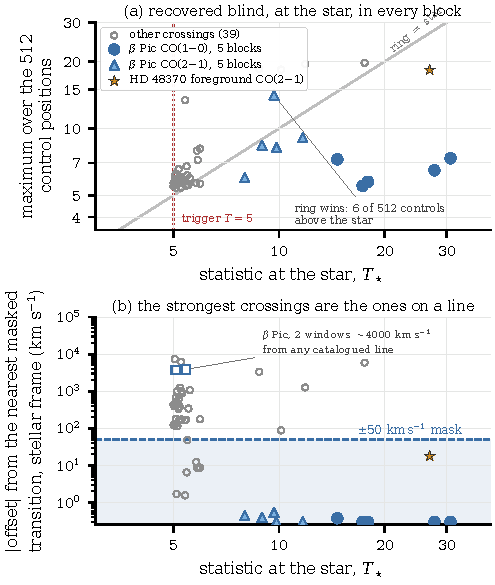
\includegraphics[width=0.88\columnwidth]{figures/bpic_control.pdf}
\caption{The $\beta$~Pictoris positive control, in both directions.
\emph{(a)}~The spatial screen. One point per execution block in which the
blind search recovers circumstellar carbon monoxide, plotted as the stellar
statistic against the maximum over that window's \NCtrl{} control positions:
the \NStageOneBpicEb{} blocks in which the star outranks every control, and
one further block in which the ring wins. \emph{The control is that the
search recovers a real narrow line at a stellar position, in two transitions
and in every one of these blocks.} It is not that the star outranks the ring
everywhere. In block \texttt{\BpCtrlBlock}, Band~\BpCtrlBand, the control
ring reaches \BpCtrlRingMax{} against \BpCtrlStar{} at the star, with
\BpCtrlNAbove{} of the \BpCtrlNCtrl{} control positions above it, so the
screen rejects a window holding carbon monoxide that is real, centred on the
star and independently mapped: \textbf{the screen measures compactness and
not authenticity} (\S\ref{sec:bpicval}). \emph{(b)}~Line confusion, which is
what makes the screen's job hard. Each crossing is plotted by its velocity
offset from the nearest masked transition \emph{in its own star's rest
frame}, with the adopted $\pm\MaskHalfKms$\,km\,s$^{-1}$ half-width
marked. The \BpicPanelNCo{} $\beta$~Pictoris carbon-monoxide crossings land
\BpicDvCoLo--\BpicDvCoHi\,km\,s$^{-1}$ from CO, at the resolution of the
systemic velocity itself, while the two CS($5{\to}4$) crossings of the same
star sit \BpicDvCsLo--\BpicDvCsHi\,km\,s$^{-1}$ from anything catalogued
and are not attributed at any width. \BpicPanelNOther{} further crossings
are drawn in grey, with HD~48370 marked; \BpicPanelNDrawn{} of the
\NCross{} are plotted, the remainder being crossings for which the release
stores no control ring. \emph{A crossing is identified by where it falls in
this plane and not by how strong it is}, which is why the line mask and not
the trigger is the productive test.}
\label{fig:bpiccontrol}
\end{figure}
